%-------------------------------------------------------------------------------
\clearpage
\section{\ttbar Sample With $h_{damp}=m_{top}$ Vs. $h_{damp}=\infty$ Comparison Study}
\label{app:hdamp_comparison}
%-------------------------------------------------------------------------------
This appendix contains a comparison study between the nominal \ttbar sample used in this analysis (with $h_{damp}$ factor set to top quark mass) and the alternative sample with $h_{damp}=\infty$ and re-weighted based on the ratio of measured differential cross sections at 7 TeV in data and MC as a function of top quark \pt and \ttbar \pt to remove discrepancies in the high top quark and \ttbar \pt regions as observed in data~\cite{topdiff_7TEV}.

\subsection{Truth fractions}
The truth helicity fractions obtained by fitting the analytical SM distribution of $\cos\theta^{*}$ to its MC distribution in full phase space. The extracted values are fully compatible as shown in table ~\ref{tab:truthFrac}.

\begin{table}[!hb]
\centering
\begin{tabular}{l|c|c|c}
\hline \hline
Sample  & $F_{0}$ & $F_{L}$ & $F_{R}$ \\ \hline\hline
$h_{damp}=\infty$ + rew. & 0.6959 & 0.3028 & 0.0013 \\
$h_{damp}=m_{top}$ 		 & 0.6956 & 0.3030 & 0.0014 \\ \hline\hline
\end{tabular}
\caption{Truth helicity fractions obtained from the MC sample's full phase space.}
\label{tab:truthFrac}
\end{table}

\subsection{Expected fractions and bias}

Table \ref{tab:rw_expectedStat_Frac_Comparison} compares the fitted helicity fractions obtained via 5000 pseudo-experiments using the nominal \ttbar sample with $h_{damp}=m_{top}$ and the alternative top quark and \ttbar \pt re-weighted sample with $h_{damp}=\infty$ in the combined electron + muon channel in one exclusive + two inclusive \bt tag region for the leptonic + hadronic channel. The shift in the central values of the expected fractions (bias) compared to the statistical + background normalization uncertainty using the nominal \ttbar sample as a reference. 

\begin{table}[!hb]
\centering
\begin{tabular}{l|c|c|c}
\hline \hline
	Sample  & $F_{0}$ & $F_{L}$ & $F_{R}$ \\ \hline\hline
	$h_{damp}=\infty$ + rew. & 0.6957 & 0.3030 & 0.0013 \\
	$h_{damp}=m_{top}$ 		 & 0.6953 & 0.3031 & 0.0015 \\ \hline
			  & $\Delta F_{0}$ & $\Delta F_{L}$ & $\Delta F_{R}$ \\ \hline
	Diff. & 0.0004 & 0.0001 & 0.0002 \\ \hline\hline
		  	  & $\sigma F_{0}$ & $\sigma F_{L}$ & $\sigma F_{R}$ \\ \hline
	Stat. + bkg. unc.	 & 0.007±1\% & 0.005±1\% & 0.004±1\% \\ \hline\hline

\end{tabular}
\caption{Expected helicity fractions and statistical + background normalization uncertainty of the helicity fractions comparison between the nominal \ttbar sample with $h_{damp}=m_{top}$ and the alternative top quark and \ttbar \pt re-weighted sample with $h_{damp}=\infty$ fitted using the combined electron + muon channel in one exclusive + two inclusive \bt tag region for the leptonic + hadronic channel.}
\label{tab:rw_expectedStat_Frac_Comparison}
\end{table}

\subsection{Data/prediction comparison}
Tables \ref{fig:rw_control_plots_1} - \ref{fig:rw_control_plots_4} compare the nominal \ttbar sample with $h_{damp}=m_{top}$ Data/prediction agreement with and the alternative top quark and \ttbar \pt re-weighted sample with $h_{damp}=\infty$ corresponding plots. The Data/prediction agreement is slightly better in the re-weighted sample. However the not re-weighted sample with $h_{damp}=m_{top}$ had been chosen as the nominal \ttbar sample in this analysis, avoiding the data driven corrections that might affect the measurement.

\begin{table}[!hb]
\centering
\begin{tabular}{c c}
	$h_{damp}=m_{top}$ & $h_{damp}=\infty$ \\
	\includegraphics[height=65mm]{figures/control_Plots2/bTag_1excl/LeptonPt_el} 	& 	\includegraphics[height=65mm]{figures/control_Plots2/bTag_1excl_rwSample/LeptonPt_el}\\
	\includegraphics[height=65mm]{figures/control_Plots2/bTag_1excl/JetPt_el} 		&	\includegraphics[height=65mm]{figures/control_Plots2/bTag_1excl_rwSample/JetPt_el}\\
	\includegraphics[height=65mm]{figures/control_Plots2/bTag_1excl/reco_Top_pt_el}	&	\includegraphics[height=65mm]{figures/control_Plots2/bTag_1excl_rwSample/reco_Top_pt_el}\\

\end{tabular}
\caption{These control plots comparing data/prediction agreement between the nominal \ttbar sample with $h_{damp}=m_{top}$ (left column) and the alternative top quark and \ttbar \pt re-weighted sample with $h_{damp}=\infty$ (right column), in the 1 exclusive \bt tag, electron channel for selected event kinematics. All plots are shown after the cut LH $> -48$.}
\label{fig:rw_control_plots_1}
\end{table}


\begin{table}[!hb]
\centering
\begin{tabular}{c c}
	$h_{damp}=m_{top}$ & $h_{damp}=\infty$ \\
	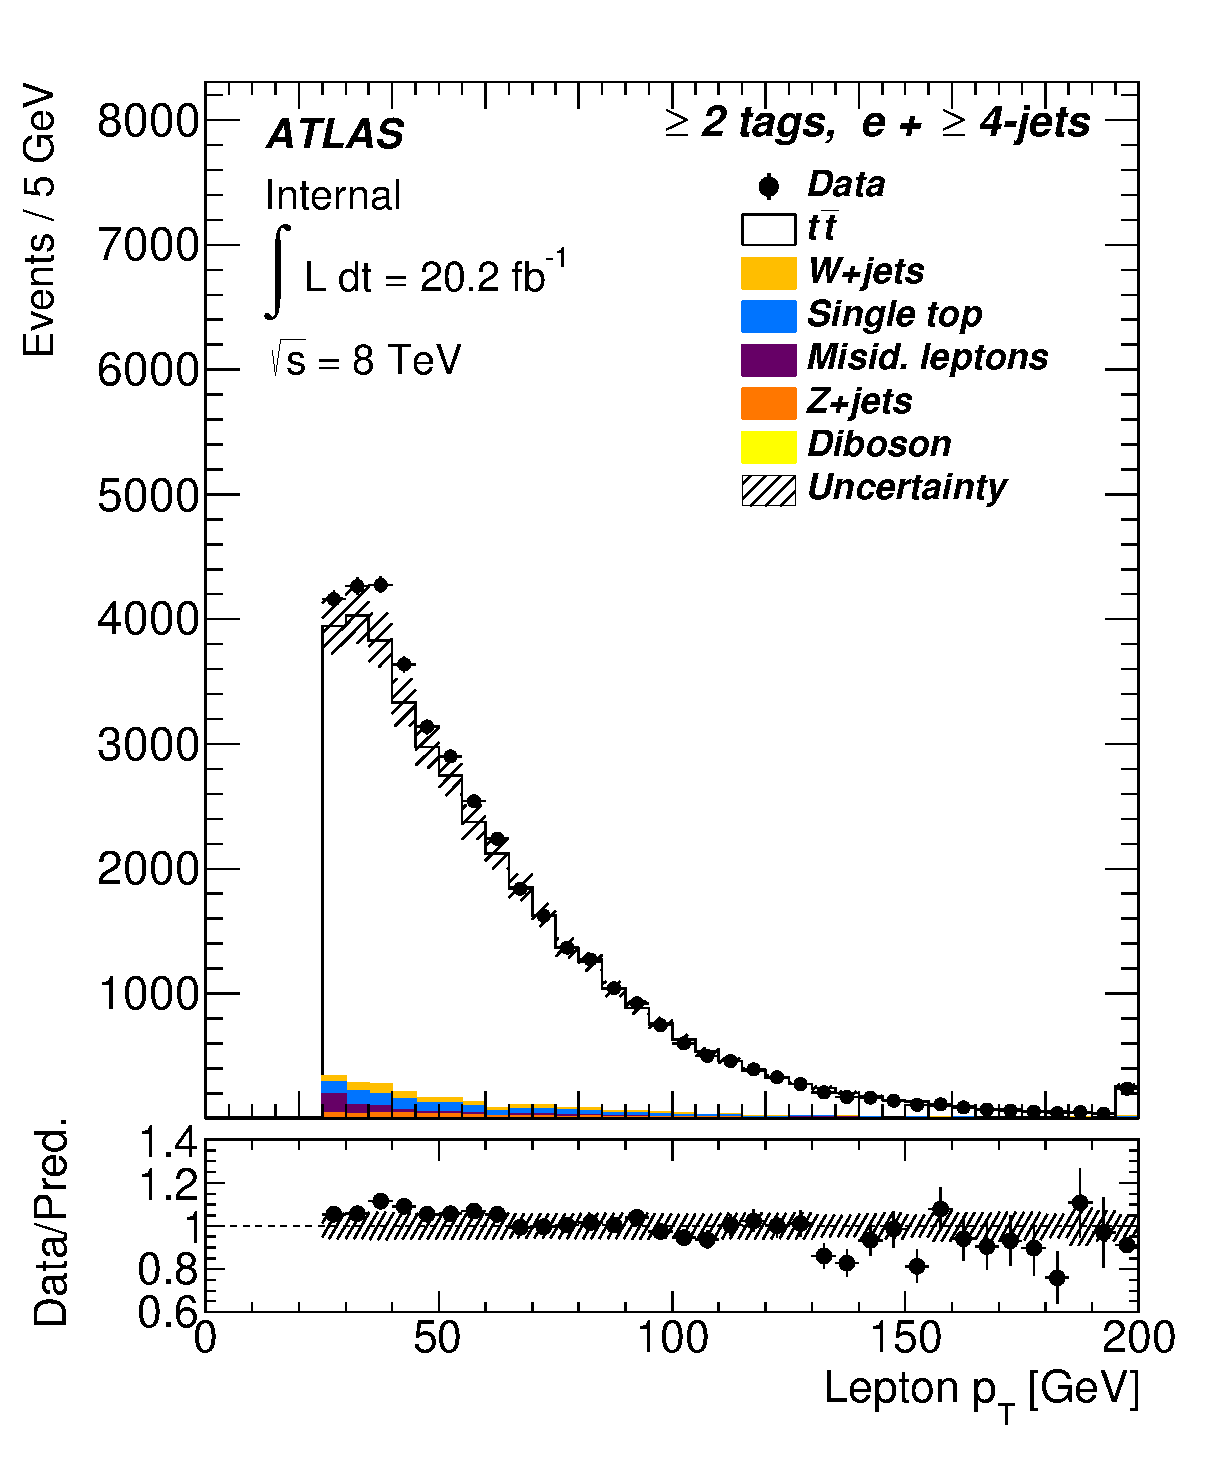
\includegraphics[height=65mm]{figures/control_Plots2/bTag_2incl/LeptonPt_el} 	& 	\includegraphics[height=65mm]{figures/control_Plots2/bTag_2incl_rwSample/LeptonPt_el}\\
	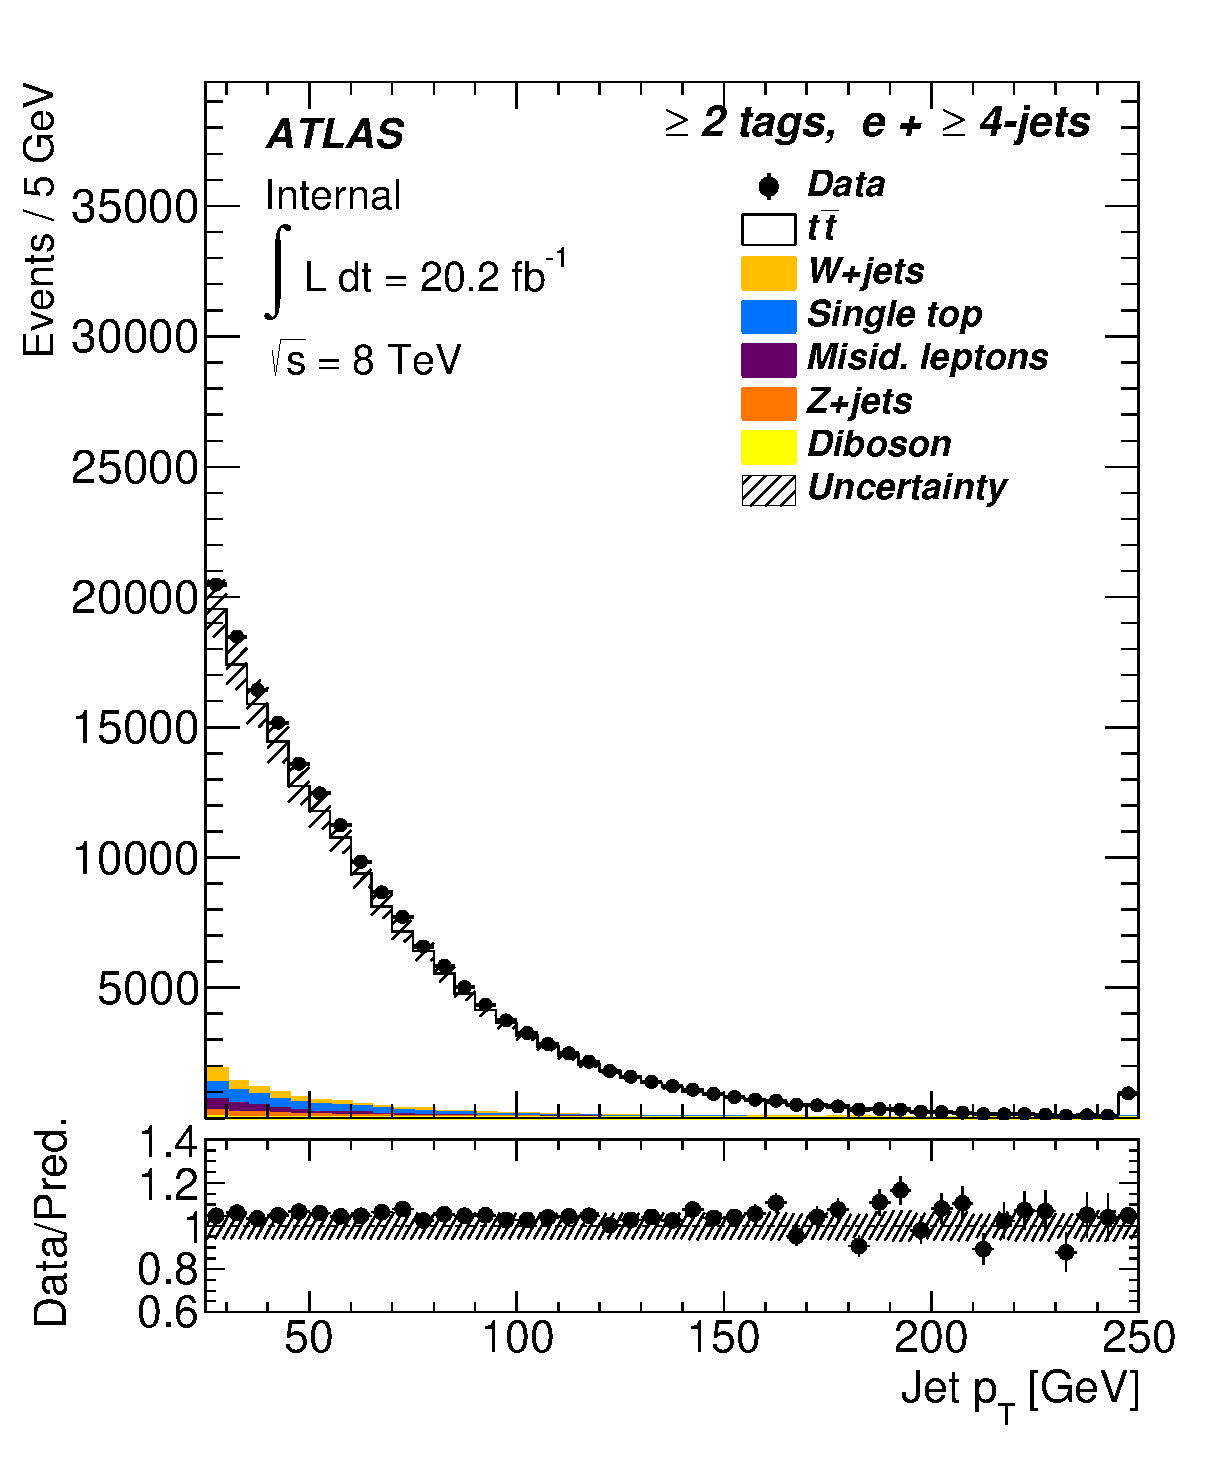
\includegraphics[height=65mm]{figures/control_Plots2/bTag_2incl/JetPt_el} 		&	\includegraphics[height=65mm]{figures/control_Plots2/bTag_2incl_rwSample/JetPt_el}\\
	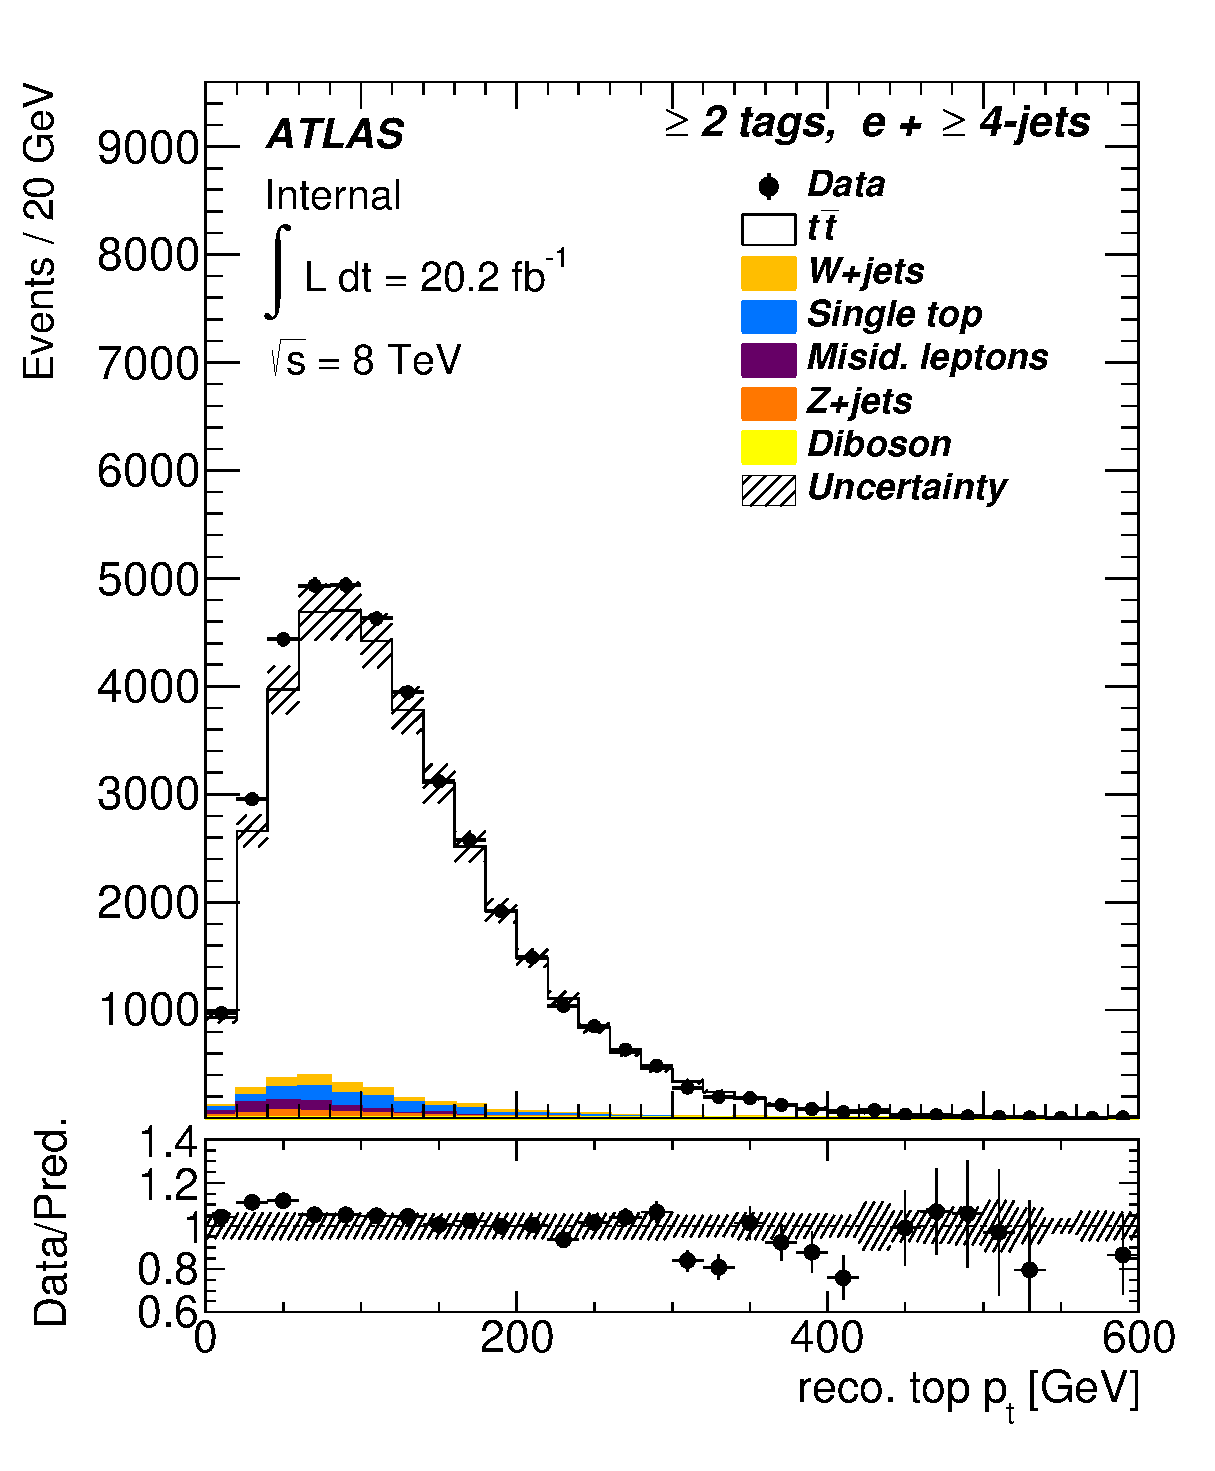
\includegraphics[height=65mm]{figures/control_Plots2/bTag_2incl/reco_Top_pt_el}	&	\includegraphics[height=65mm]{figures/control_Plots2/bTag_2incl_rwSample/reco_Top_pt_el}\\

\end{tabular}
\caption{These control plots comparing data/prediction agreement between the nominal \ttbar sample with $h_{damp}=m_{top}$ (left column) and the alternative top quark and \ttbar \pt re-weighted sample with $h_{damp}=\infty$ (right column), in the 2 inclusive \bt tag, electron channel for selected event kinematics. All plots are shown after the cut LH $> -48$.}
\label{fig:rw_control_plots_2}
\end{table}

\begin{table}[!hb]
\centering
\begin{tabular}{c c}
	$h_{damp}=m_{top}$ & $h_{damp}=\infty$ \\
	\includegraphics[height=65mm]{figures/control_Plots2/bTag_1excl/LeptonPt_mu} 	& 	\includegraphics[height=65mm]{figures/control_Plots2/bTag_1excl_rwSample/LeptonPt_mu}\\
	\includegraphics[height=65mm]{figures/control_Plots2/bTag_1excl/JetPt_mu} 		&	\includegraphics[height=65mm]{figures/control_Plots2/bTag_1excl_rwSample/JetPt_mu}\\
	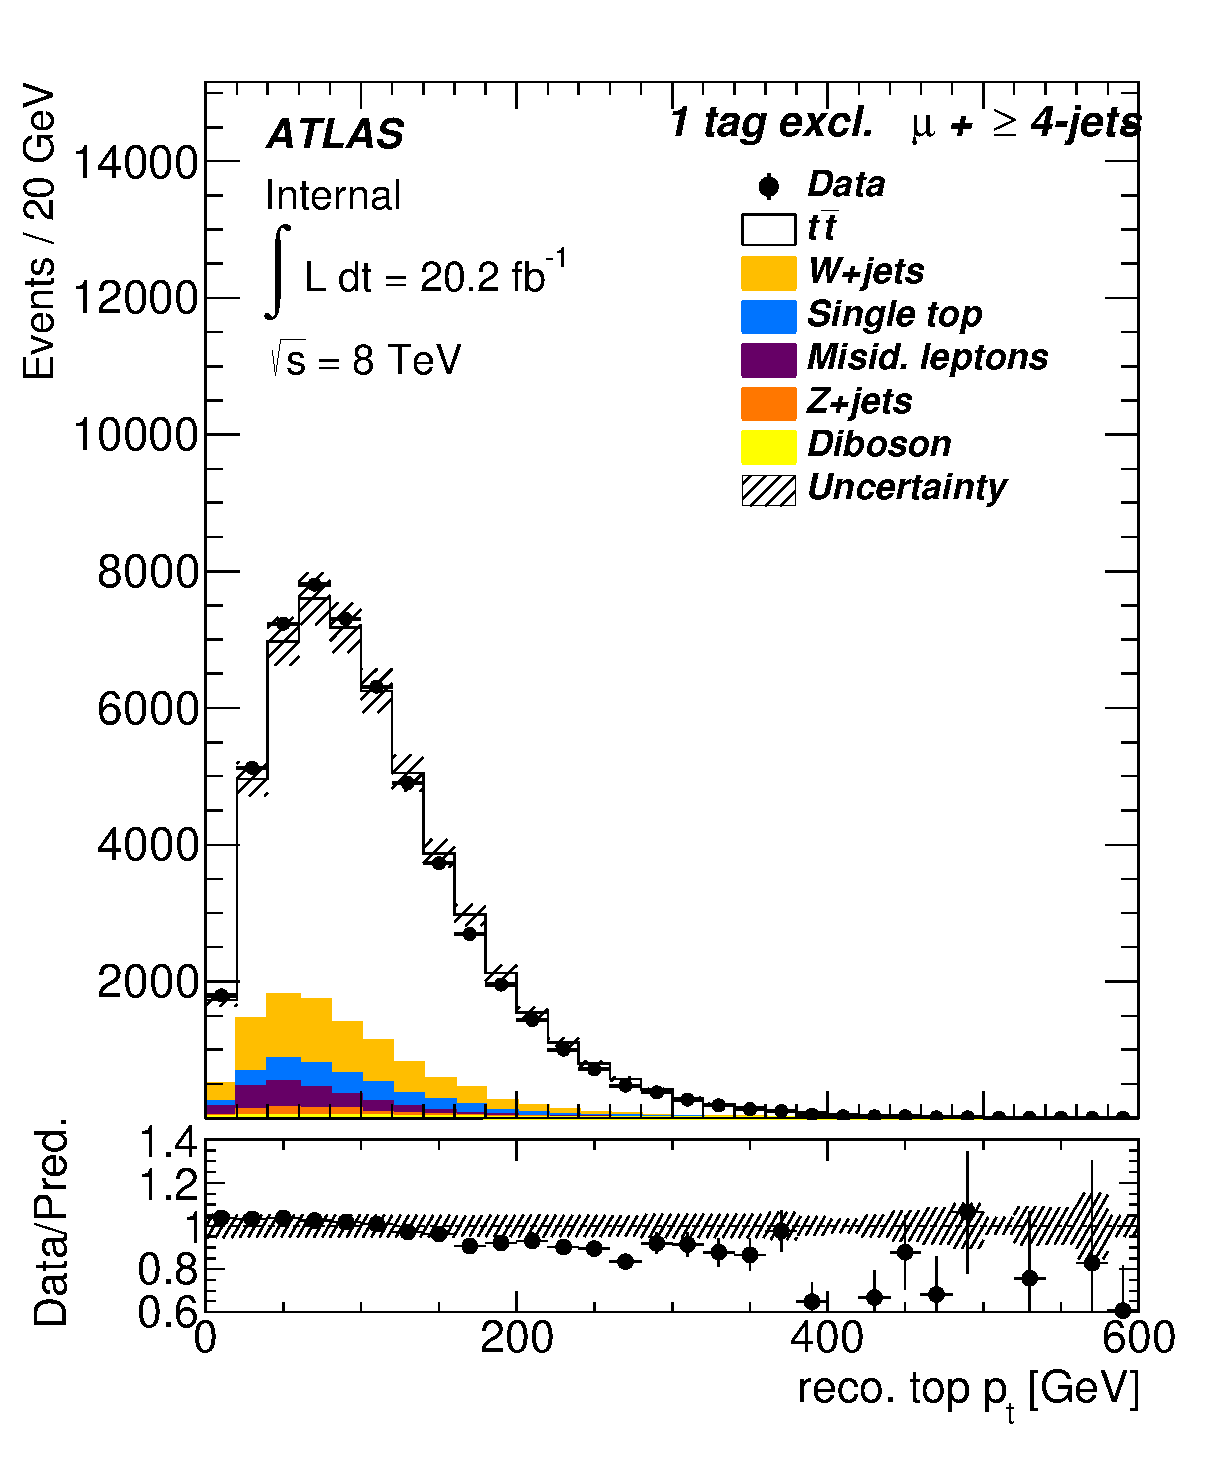
\includegraphics[height=65mm]{figures/control_Plots2/bTag_1excl/reco_Top_pt_mu}	&	\includegraphics[height=65mm]{figures/control_Plots2/bTag_1excl_rwSample/reco_Top_pt_mu}\\

\end{tabular}
\caption{These control plots comparing data/prediction agreement between the nominal \ttbar sample with $h_{damp}=m_{top}$ (left column) and the alternative top quark and \ttbar \pt re-weighted sample with $h_{damp}=\infty$ (right column), in the 1 exclusive \bt tag, muon channel for selected event kinematics. All plots are shown after the cut LH $> -48$.}
\label{fig:rw_control_plots_3}
\end{table}

\begin{table}[!hb]
\centering
\begin{tabular}{c c}
	$h_{damp}=m_{top}$ & $h_{damp}=\infty$ \\
	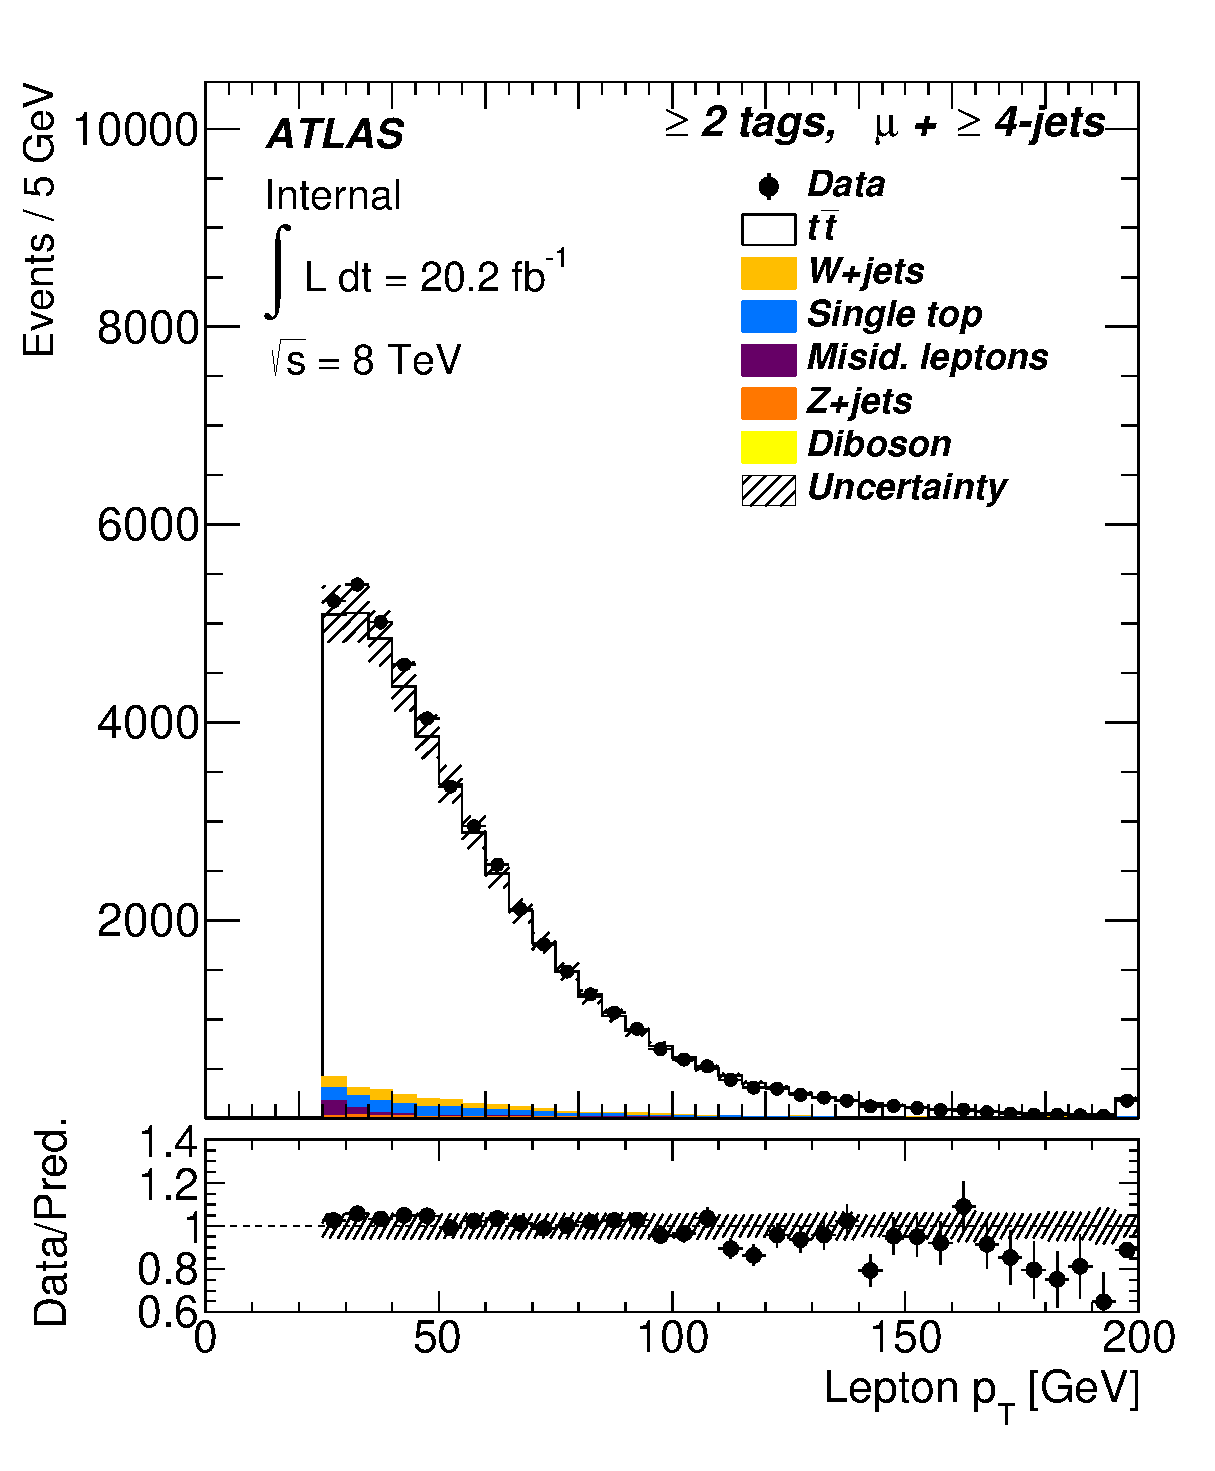
\includegraphics[height=65mm]{figures/control_Plots2/bTag_2incl/LeptonPt_mu} 	& 	\includegraphics[height=65mm]{figures/control_Plots2/bTag_2incl_rwSample/LeptonPt_mu}\\
	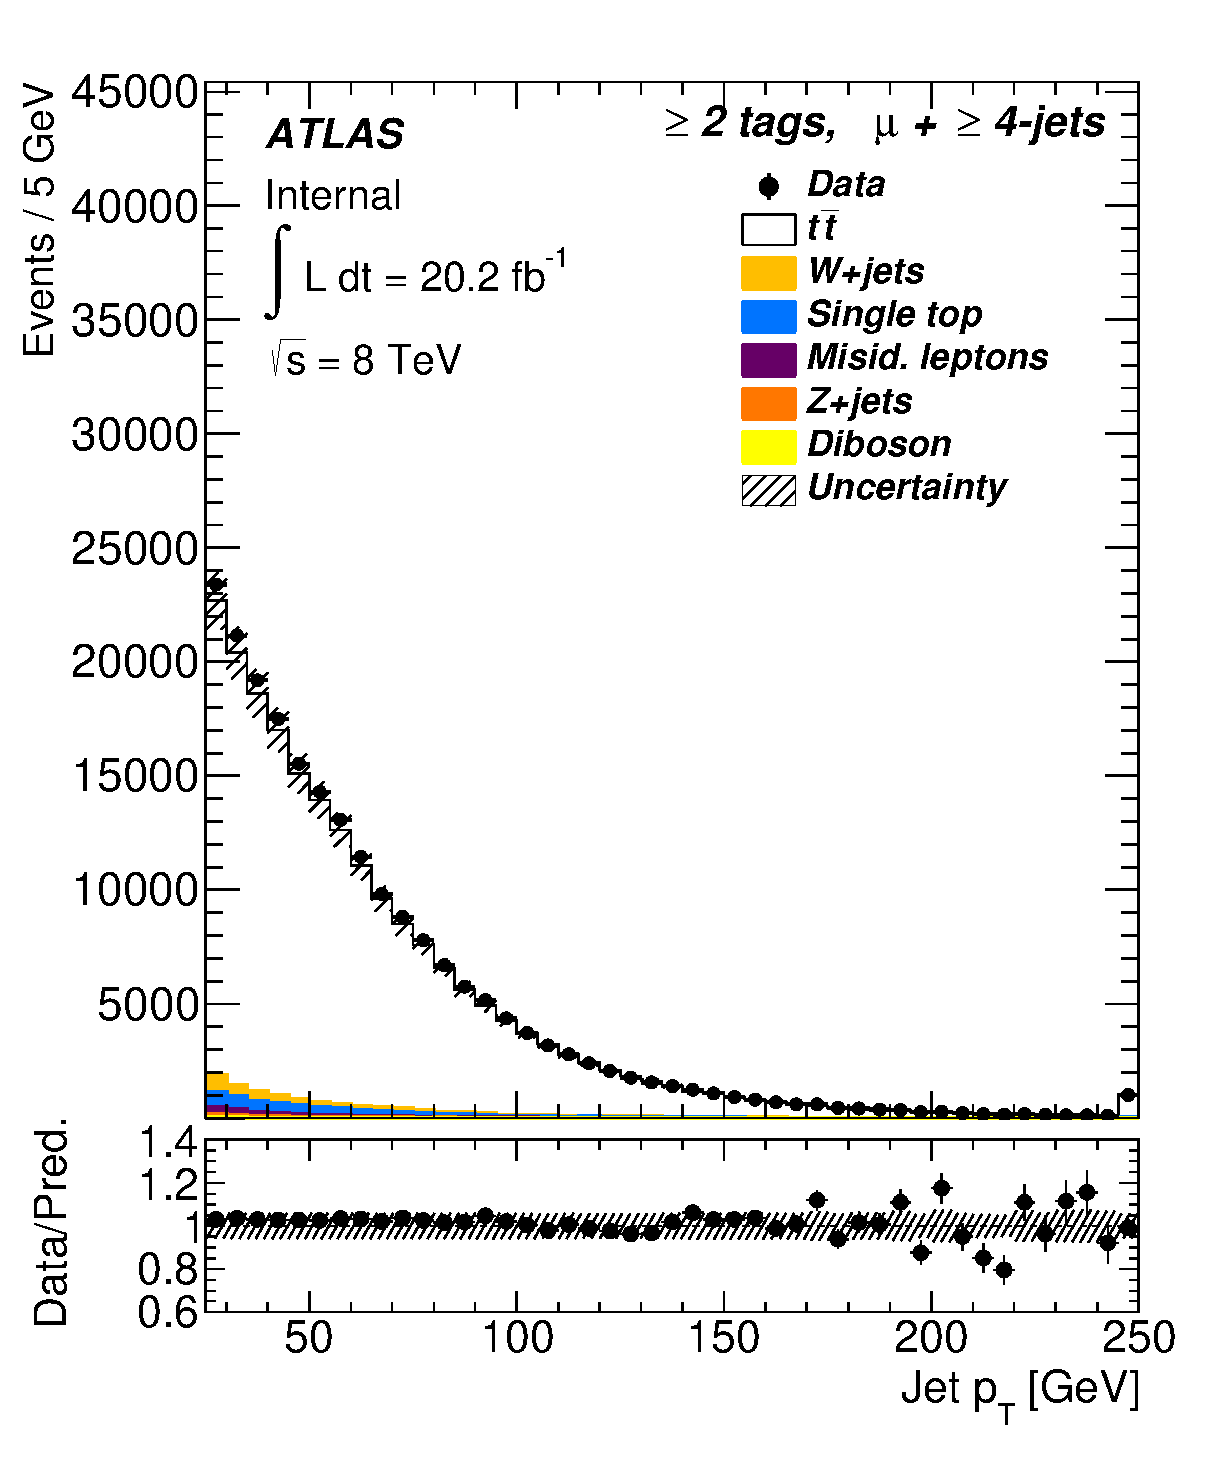
\includegraphics[height=65mm]{figures/control_Plots2/bTag_2incl/JetPt_mu} 		&	\includegraphics[height=65mm]{figures/control_Plots2/bTag_2incl_rwSample/JetPt_mu}\\
	\includegraphics[height=65mm]{figures/control_Plots2/bTag_2incl/reco_Top_pt_mu}	&	\includegraphics[height=65mm]{figures/control_Plots2/bTag_2incl_rwSample/reco_Top_pt_mu}\\

\end{tabular}
\caption{These control plots comparing data/prediction agreement between the nominal \ttbar sample with $h_{damp}=m_{top}$ (left column) and the alternative top quark and \ttbar \pt re-weighted sample with $h_{damp}=\infty$ (right column), in the 2 inclusive \bt tag, muon channel for selected event kinematics. All plots are shown after the cut LH $> -48$.}
\label{fig:rw_control_plots_4}
\end{table}




